\documentclass{article}
\usepackage[final]{neurips_2023}

\usepackage[utf8]{inputenc} % allow utf-8 input
\usepackage[T1]{fontenc}    % use 8-bit T1 fonts
\usepackage{hyperref}       % hyperlinks
\usepackage{url}            % simple URL typesetting
\usepackage{booktabs}       % professional-quality tables
\usepackage{amsfonts}       % blackboard math symbols
\usepackage{nicefrac}       % compact symbols for 1/2, etc.
\usepackage{microtype}      % microtypography
\usepackage{xcolor}         % colors
\usepackage{authblk}
\usepackage{graphicx}
\usepackage{lipsum}         % for filler text if needed

\title{Privacy Ranker: Assessing Privacy Risk in Social Media Profiles}

\author[1]{Justin Hoyle}
\author[2]{Matthew Glennon}
\author[3]{Jay Darshitbhai Patel}

\affil[1,2,3]{Virginia Commonwealth University}
\affil[1]{\texttt{hoylejb2@vcu.edu}}
\affil[2]{\texttt{mglennon@vcu.edu}}
\affil[3]{\texttt{patelj33@vcu.edu}}

\begin{document}

\maketitle

\begin{abstract}
This project aims to develop a Privacy Ranker that evaluates and ranks users’ social media profiles based on their privacy risk. Many users unknowingly expose Personally Identifiable Information (PII) on platforms such as Twitter, LinkedIn, and Instagram, leading to privacy leaks, identity theft, and more. Our approach leverages a combination of natural language processing and machine learning techniques to extract PII from raw textual data and to assess the associated privacy risk.
\end{abstract}

\section{Introduction}
In today's digital era, social media platforms are ubiquitous channels for communication and self-expression. However, the ease of sharing information often leads to unintended exposure of sensitive data. This exposure can increase the risk of identity theft, phishing, and unauthorized data aggregation. Our project addresses these challenges by developing a system—the \emph{Privacy Ranker}—that automatically identifies PII in social media posts and assigns a privacy risk score based on the volume and type of exposed information.

\section{Data Source}
The primary dataset used in this project is the Sentiment140 dataset (\url{https://www.kaggle.com/datasets/kazanova/sentiment140}), originally designed for sentiment analysis. Despite its original purpose, the rich textual content of tweets makes this dataset an excellent candidate for evaluating privacy risks. To tailor the dataset for our analysis, additional annotations have been introduced to label and highlight PII, which serve as inputs for subsequent processing stages.

\section{Methodology}
The overall pipeline of the Privacy Ranker comprises several key stages. Each stage is implemented in separate Python scripts, as described below.

\subsection{Data Cleaning}
Data cleaning is implemented in \texttt{clean\_csv.py}. The process consists of:
\begin{itemize}
    \item \textbf{CSV Parsing:} The dataset is read using \texttt{pandas} with the proper encoding (``latin-1'').
    \item \textbf{Column Reduction:} The raw CSV file contains several columns; the script drops columns with indices 0, 2, and 3, retaining only the tweet ID, user identifier, and tweet text.
    \item \textbf{Data Quality Assurance:} After renaming the remaining columns to \texttt{ids}, \texttt{user}, and \texttt{text}, empty entries and duplicate tweets are removed.
    \item \textbf{Text Cleaning:} A custom function \texttt{clean\_text()} converts text to lowercase and uses regular expressions to strip URLs, mentions, hashtags, punctuation, and common stopwords (via NLTK).
    \item \textbf{Mention Filtering:} The \texttt{remove\_mentions()} function filters out rows where PII tags include mentions (e.g., \texttt{PERSON: @} tags) and writes the filtered data to the output CSV.
\end{itemize}

\subsection{Computational Infrastructure}
The NER extraction and model training steps leverage the Apollo cluster at Virginia Commonwealth University’s High Performance Research Computing (HPRC) facility. The provided \texttt{NER\_slurm.sh} script dispatches the NER pipeline to the cluster with a Slurm job requesting 1 GPU, 4 CPUs, and 32 GB of memory, logging output to \texttt{hf\_ner\_\%j.out}. Sentence embeddings generation and Random Forest training were performed on nodes equipped with Nvidia P100 GPUs and high-memory configurations. The Apollo cluster comprises 18 compute nodes with 604 CPUs, 5.9 TB of RAM, 3 PB of Lustre storage, and 54 Gb/s InfiniBand interconnect.

\subsection{Named Entity Recognition for PII Extraction}
The extraction of PII is implemented in \texttt{named\_entity\_recognition.py} using Hugging Face’s \texttt{transformers} library. The script loads the \texttt{Jean-Baptiste/roberta-large-ner-english} model and tokenizer into a grouped-entity NER pipeline. Each tweet is processed to detect entities in the categories \texttt{PER}, \texttt{ORG}, \texttt{LOC}, and \texttt{MISC}, producing a comma-separated list of PII tags per tweet. The results are written to \texttt{pii\_detected\_tweets.csv}. GPU acceleration is available when running via the \texttt{NER\_slurm.sh} script.

\subsection{Feature Engineering and Machine Learning}
The project implements a classical machine learning pipeline centered on a Random Forest classifier. Text representations are generated using sentence embeddings from the \texttt{all-MiniLM-L6-v2} model via the \texttt{SentenceTransformer} library. Structured features include binary indicators for PII categories (\texttt{has\_per}, \texttt{has\_org}, \texttt{has\_loc}, \texttt{has\_misc}), \texttt{text\_length}, and \texttt{word\_count}. The text embeddings and structured features are concatenated to form the final feature matrix. After oversampling the minority classes with SMOTE, a Random Forest model (max depth 20, 200 estimators, balanced class weights) is trained on the resampled data.

\subsection{Model Training and Evaluation}
The Random Forest classifier is trained on the SMOTE-resampled data. Evaluation uses:
\begin{itemize}
    \item \textbf{Classification Report:} Precision, recall, and F1-score metrics.
    \item \textbf{Confusion Matrix:} Visualization of true versus predicted risk labels.
\end{itemize}
After evaluation, both the trained Random Forest model and the sentence embedding encoder are serialized via \texttt{joblib} (to \texttt{random\_forest\_model\_embed.pkl} and \texttt{sentence\_transformer\_embedder.pkl}, respectively).

\subsection{Model Testing}
The \texttt{test\_model.py} script loads the serialized Random Forest model and the saved vectorizer. For each new input, it computes structured features (\texttt{has\_email}, \texttt{has\_phone}, \texttt{has\_person}, \texttt{has\_org}, \texttt{has\_gpe}, \texttt{text\_length}, \texttt{word\_count}) and applies the vectorizer to encode the raw text. The script concatenates the resulting text vectors with structured features to form the test feature matrix, performs inference to predict risk labels, and optionally generates a classification report comparing predictions to true labels.

\section{Experimental Setup and Results}
The experiments were conducted on a standard workstation. Key aspects include:
\begin{itemize}
    \item \textbf{Train-Test Split:} An 80/20 split was employed to create the training and test sets.
    \item \textbf{Oversampling:} SMOTE was applied to the training data to balance the distribution of risk labels.
    \item \textbf{Model Configuration:} The Random Forest classifier was configured with a maximum depth of 20, 200 estimators, and balanced class weights.
\end{itemize}

\begin{figure}[ht]
    \centering
    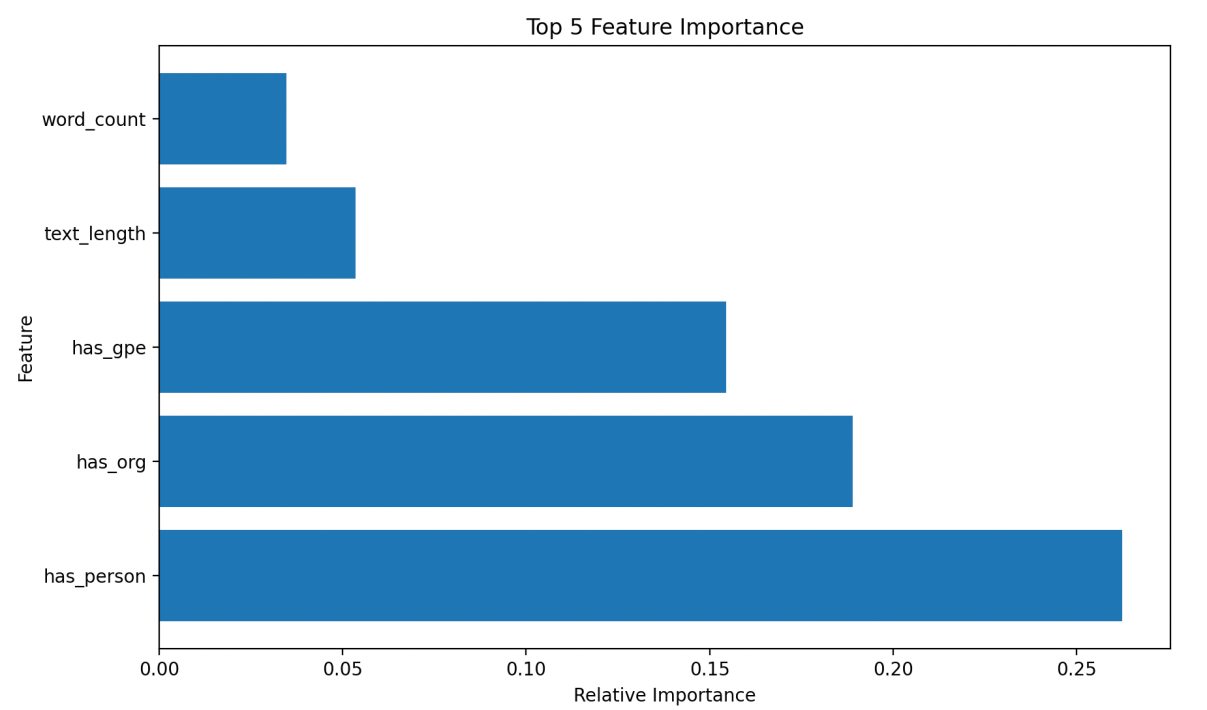
\includegraphics[width=0.6\linewidth]{fi.png}
    \caption{Top 5 Feature Importance in the Random Forest Classifier.}
    \label{fig:feature_importance}
\end{figure}

\begin{figure}[ht]
    \centering
    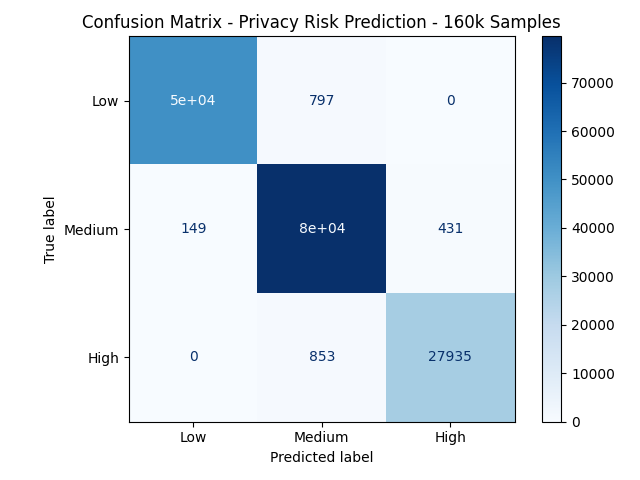
\includegraphics[width=0.6\linewidth]{cm.png}
    \caption{Confusion matrix for the Random Forest classifier on the test set.}
    \label{fig:confusion}
\end{figure}

\section{Discussion}
Our implementation demonstrates a systematic approach to privacy risk assessment:
\begin{itemize}
    \item The dual approach for PII extraction—combining Hugging Face’s transformer-based NER with regular expressions—ensures that a wide variety of PII is captured.
    \item Data cleaning and preprocessing steps are essential to reduce noise and improve the quality of input data.
    \item Feature engineering, which includes both text-based features and structured indicators, provides a comprehensive representation of the data.
    \item The use of SMOTE to mitigate class imbalance significantly contributes to the robustness of the trained Random Forest classifier.
\end{itemize}
The modular design, with distinct scripts for cleaning, extraction, feature processing, and model testing, facilitates easier debugging and future enhancements.

\section{Conclusion and Future Work}
This paper presented an end-to-end framework for assessing privacy risks in social media profiles by detecting and classifying PII. The Privacy Ranker system integrates robust data preprocessing, advanced PII extraction using Hugging Face’s transformers, comprehensive feature engineering, and a classical Random Forest model to generate actionable risk scores.

Future work may include:
\begin{itemize}
    \item Integrating more advanced deep learning models for both text representation and risk prediction.
    \item Expanding the dataset to include additional social media platforms and non-English languages.
    \item Conducting user studies to further validate the practical utility of the Privacy Ranker in real-world scenarios.
    \item Exploring the adaptability of the system to various deployment constraints by leveraging multiple modeling paradigms.
\end{itemize}

\section{Code Repository}
The complete codebase for this project is available at:
\url{https://github.com/JustinHoyle/Final-Project-CMSC-512}

The repository includes:
\begin{itemize}
    \item \texttt{clean\_csv.py}: Cleans raw CSV, applies text preprocessing, and filters out PII mentions with \texttt{remove\_mentions()}.
    \item \texttt{named\_entity\_recognition.py}: Performs NER-based PII extraction via a Hugging Face pipeline.
    \item \texttt{NER\_slurm.sh}: Slurm job script to run the NER pipeline on a GPU-enabled HPC node.
    \item \texttt{feature\_processing.py}: Generates sentence embeddings, assembles structured features, applies SMOTE, trains a Random Forest classifier, and saves the model and embedder.
    \item \texttt{test\_model.py}: Loads the saved model and vectorizer, computes features for new data, and outputs risk predictions and evaluation metrics.
    \item Serialized artifacts in \texttt{models/}: \texttt{random\_forest\_model\_embed.pkl}, \texttt{sentence\_transformer\_embedder.pkl}, and \texttt{tfidf\_vectorizer.pkl}.
    \item Additional exploratory notebooks and utility scripts.
\end{itemize}

\section*{References}
\begin{itemize}
    \item \texttt{pandas} documentation: \url{https://pandas.pydata.org/}
    \item \texttt{nltk} documentation: \url{https://www.nltk.org/}
    \item \texttt{transformers} library: \url{https://huggingface.co/docs/transformers/}
    \item \texttt{sentence-transformers} documentation: \url{https://www.sbert.net/}
    \item \texttt{scikit-learn} documentation: \url{https://scikit-learn.org/}
    \item \texttt{imbalanced-learn} (SMOTE): \url{https://imbalanced-learn.org/}
\end{itemize}

\newpage
\appendix

\section{Appendix: Hyperparameter Settings and Additional Results}

\subsection{Random Forest Hyperparameters}
\begin{table}[ht]
    \centering
    \begin{tabular}{ll}
        \toprule
        Parameter             & Value \\
        \midrule
        Number of Trees       & 200 \\
        Max Depth             & 20 \\
        Max Features          & sqrt \\
        Min Samples Leaf      & 4 \\
        Min Samples Split     & 10 \\
        Class Weight          & balanced \\
        Random State          & 42 \\
        \bottomrule
    \end{tabular}
    \caption{Random Forest hyperparameter settings.}
\end{table}

\subsection{Additional Experimental Results}
\begin{figure}[ht]
    \centering
    \includegraphics[width=0.6\linewidth]{roc_curve.png}
    \caption{ROC curve for the Random Forest classifier on the test set.}
    \label{fig:roc}
\end{figure}

\end{document}